% Packages

\documentclass[12pt]{article}
\usepackage[letterpaper, margin=1in, utf8]{geometry}
\usepackage{fancyhdr, graphicx, xcolor, wrapfig, hyperref}
\usepackage[thinlines]{easytable}
\graphicspath{ {./images/} }


\pagestyle{fancy} % Utilisation de fancyhdr

% -------------------------

% Première page

\title{\Huge\textbf{Quack - Jeu d'échec scolaire}}
\date{Juin 2025}

% -------------------------

\begin{document}
\maketitle

% Mise en page footer / header

\renewcommand{\headrulewidth}{0mm} % Vire la ligne du header
\renewcommand{\footrulewidth}{0.1mm} % Redimensionne la ligne du footer
\rhead{QUACK}
\lfoot{EPITA 2027}

% ------------------------------

\centerline{Groupe 2}
\vspace{\fill}
Lépine Marc-Aurèle \par
Battistella Alexis \par
Loup Thomas \par
Maston Claudia \par
Delrieu Nathan

% Nom du groupe

% /-------------------\
% | Début du Document |
% \-------------------/

\newpage

\renewcommand\contentsname{\centering Table des matières}
% Remplace le nom par défaut de la Table des matières
\renewcommand\footnoterule{}
% Supprime la ligne séparatrice des footnotes

\tableofcontents
% Créé une table des matières à partir des sections, subsections et subsubsections

\newpage

\section{Introduction}
    Ce projet est un projet. Voilà bonne journée.
  
\section {Description}
    \subsection{Découpage de la grille}
    Nous avons choisi de découper la grille de manière récursive de telle sorte à pouvoir travailler de manière récursive sur des grilles 2x2 comme celle-ci :

    \label{sec:grid-2x2}
    \begin{center}
        \begin{TAB}(4,2cm,2cm, 2cm, 2cm)[5pt]{|c|c|}{|c|c|}% (rows,min,max)[tabcolsep]{columns {rows}
            00 & 01 \\
            10 & 11 \\
        \end{TAB}
    \end{center}

    \subsubsection{Grille 4x4}
    \begin{center}
        \begin{TAB}(4,2cm,2cm, 2cm, 2cm)[5pt]{|c|c|c|c|}{|c|c|c|c|}% (rows,min,max)[tabcolsep]{columns}{rows}
        \textcolor{red}{00}00 & \textcolor{red}{00}01 & \textcolor{red}{01}00 & \textcolor{red}{01}01 \\
        \textcolor{red}{00}10 & \textcolor{red}{00}11 & \textcolor{red}{01}10 & \textcolor{red}{01}11 \\
        \textcolor{red}{10}00 & \textcolor{red}{10}01 & \textcolor{red}{11}00 & \textcolor{red}{11}01 \\
        \textcolor{red}{10}10 & \textcolor{red}{10}11 & \textcolor{red}{11}10 & \textcolor{red}{11}11 \\
        \end{TAB}
    \end{center}

    Les deux Qbits en \textcolor{red}{rouge} donnent la position de la sous-grille et les deux noirs donnent la position de la clé dans la sous-grille.

    \subsubsection{Grille 8x8}


    \newpage
    Le principe est exactement le même pour la version 8x8 (c'est juste moins lisible ;-;).
        \begin{center}
        \begin{TAB}(4,2cm,2cm, 2cm, 2cm)[5pt]{|c|c|c|c|c|c|c|c|}{|c|c|c|c|c|c|c|c|}% (rows,min,max)[tabcolsep]{columns}{rows}
        \textcolor{red}{00}\textcolor{blue}{00}000 & \textcolor{red}{00}\textcolor{blue}{00}01 & \textcolor{red}{00}\textcolor{blue}{01}00 & \textcolor{red}{00}\textcolor{blue}{01}01 & \textcolor{red}{01}\textcolor{blue}{00}00 & \textcolor{red}{01}\textcolor{blue}{00}01 & \textcolor{red}{01}\textcolor{blue}{01}00 & \textcolor{red}{01}\textcolor{blue}{01}01 \\
        \textcolor{red}{00}\textcolor{blue}{00}10 & \textcolor{red}{00}\textcolor{blue}{00}11 & \textcolor{red}{00}\textcolor{blue}{01}10 & \textcolor{red}{00}\textcolor{blue}{01}11 & \textcolor{red}{01}\textcolor{blue}{00}10 & \textcolor{red}{01}\textcolor{blue}{00}11 & \textcolor{red}{01}\textcolor{blue}{01}10 & \textcolor{red}{01}\textcolor{blue}{01}11 \\
        \textcolor{red}{00}\textcolor{blue}{10}00 & \textcolor{red}{00}\textcolor{blue}{10}01 & \textcolor{red}{00}\textcolor{blue}{11}00 & \textcolor{red}{00}\textcolor{blue}{11}01 & \textcolor{red}{01}\textcolor{blue}{10}00 & \textcolor{red}{01}\textcolor{blue}{10}01 & \textcolor{red}{01}\textcolor{blue}{11}00 & \textcolor{red}{01}\textcolor{blue}{11}01 \\
        \textcolor{red}{00}\textcolor{blue}{10}10 & \textcolor{red}{00}\textcolor{blue}{10}11 & \textcolor{red}{00}\textcolor{blue}{11}10 & \textcolor{red}{00}\textcolor{blue}{11}11 & \textcolor{red}{01}\textcolor{blue}{10}10 & \textcolor{red}{01}\textcolor{blue}{10}11 & \textcolor{red}{01}\textcolor{blue}{11}10 & \textcolor{red}{01}\textcolor{blue}{11}11 \\
        \textcolor{red}{10}\textcolor{blue}{00}00 & \textcolor{red}{10}\textcolor{blue}{00}01 & \textcolor{red}{10}\textcolor{blue}{01}00 & \textcolor{red}{10}\textcolor{blue}{01}01 & \textcolor{red}{11}\textcolor{blue}{00}00 & \textcolor{red}{11}\textcolor{blue}{00}01 & \textcolor{red}{11}\textcolor{blue}{01}00 & \textcolor{red}{11}\textcolor{blue}{01}01 \\
        \textcolor{red}{10}\textcolor{blue}{00}10 & \textcolor{red}{10}\textcolor{blue}{00}11 & \textcolor{red}{10}\textcolor{blue}{01}10 & \textcolor{red}{10}\textcolor{blue}{01}11 & \textcolor{red}{11}\textcolor{blue}{00}10 & \textcolor{red}{11}\textcolor{blue}{00}11 & \textcolor{red}{11}\textcolor{blue}{01}10 & \textcolor{red}{11}\textcolor{blue}{01}11 \\
        \textcolor{red}{10}\textcolor{blue}{10}00 & \textcolor{red}{10}\textcolor{blue}{10}01 & \textcolor{red}{10}\textcolor{blue}{11}00 & \textcolor{red}{10}\textcolor{blue}{11}01 & \textcolor{red}{11}\textcolor{blue}{10}00 & \textcolor{red}{11}\textcolor{blue}{10}01 & \textcolor{red}{11}\textcolor{blue}{11}00 & \textcolor{red}{11}\textcolor{blue}{11}01 \\
        \textcolor{red}{10}\textcolor{blue}{10}10 & \textcolor{red}{10}\textcolor{blue}{10}11 & \textcolor{red}{10}\textcolor{blue}{11}10 & \textcolor{red}{10}\textcolor{blue}{11}11 & \textcolor{red}{11}\textcolor{blue}{10}10 & \textcolor{red}{11}\textcolor{blue}{10}11 & \textcolor{red}{11}\textcolor{blue}{11}10 & \textcolor{red}{11}\textcolor{blue}{11}11 \\
        \end{TAB}
    \end{center}

    Les deux Qbits en \textcolor{red}{rouge} donnent la position de la 1re sous-grille, les \textcolor{blue}{bleus} celle de la 2e sous-grille, et les deux noirs la position de la clé.

    \newpage
    \subsection{Description des Q-bits}

    \begin{wrapfigure}{l}{0.5\textwidth}
        \begin{center}
            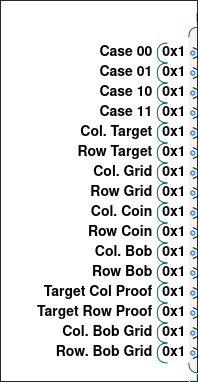
\includegraphics[width=0.8\linewidth]{image.png}
            \caption{Q-Bits}
            \label{fig:enter-label}
        \end{center}
    \end{wrapfigure}
    L'on dispose de 4 Q-bits représentant 4 cases (cf. \hyperref[sec:grid-2x2]{section 2.1}).
    \vspace{5mm}
    
    Les Q-bits \textbf{Col.Target} et \textbf{Row.Target} représentent la position de la case ciblée. Dans le cas d'une grille 4x4, target représentera premièrement la sous-grille dans laquelle se trouve la clé, puis dans un second temps la case dans laquelle ce trouve la clé. La concaténation des deux tirages de Target nous donnent les 4 bits de la position de la clé.
    
    \vspace{5mm}

    Les Q-bits \textbf{Col.Grid} et \textbf{Row.Grid} donnent la position de la sous-grille où le jeton doit être flip. Nous avons abitrairement choisi la sous grille en bas à gauche. Ainsi, Alice devra flip le coin en \textbf{11XY} où X est donné par \textbf{Row.Grid} et Y par \textbf{Col.Grid}.

    \vspace{5mm}

    De manière analogue, \textbf{Row.Coin} et \textbf{Col.Coin} représentent respectivement le bit \textbf{X} et \textbf{Y} de la case à la position \textbf{00XY} de la pièce à tourner.

    \vspace{5mm}

    Enfin, les Q-bits \textbf{Row.Bob.Grid} et \textbf{Col.Bob.Grid}, \textbf{Row.Bob} et \textbf{Col.Bob} donnent de les composantes X et Y des deux coins que Bob doit flip respectivement en bas à droite (\textbf{11XY}) et en haut à gauche (\textbf{00XY}).

    \vspace{5mm}
    Notez que les Q-bits \textbf{Target Col Proof} et \textbf{Target Row Proof} servent uniquement à vérifier la justesse de \textbf{Col.Bob.Grid} et \textbf{Row.Bob.Grid} lors du tirage de la sous-grille.
    De même, \textbf{Col.Target} et \textbf{Row.Target} sont mesurés pour vérifier la justesse de \textbf{Col.Bob} et \textbf{Row.Bob}.

    \vspace{10mm}
    Comme vu ci-dessus, le pattern est scalable à une grille 8x8. Pour celà, il nous faudra simplement une paire de Q-bits en plus représentant la position dans la 2e sous-grille, et le choix arbitraire d'un coin de l'échiquier.

    \section{Analyse mathématique}
    \section{Conclusion}
\end{document}
